\chapter{Explicaciones}
\label{cap:explicaciones}

El objetivo de nuestro trabajo consiste en explicar las relaciones entre dos canciones dadas por un recomendador de música que trabaja con un dataset concreto. De esta manera, llamaremos \textbf{explicación} a cada factor común que compartan ambas canciones, siendo principalmente propiedades que poseen las propias canciones o los valores de otras propiedades intermedias. A lo largo de este capítulo concretaremos todas las explicaciones que vamos a estudiar y el sistema que une todas ellas para poder relacionar dos canciones en su totalidad.\\

Las relaciones que recogemos en cualquier caso de uso forman un grafo siguiendo el modelo RDF. Hemos decidido, además de seguir ese formato, dotarlas de un nivel que escala a medida que el estudio se aleje del objeto canción inicial. Al expresar alejamiento, nos referimos a que, como en el contexto del formato RDF y Linked Data, la creación de relaciones se establece navegando por distintos objetos relacionados con el inicial secuencialmente. La idea de los niveles viene dada por dos motivos:\\

El primero es debido a la cercanía de niveles. Cuanto menor sea el nivel, significará que está mas próximo al objeto canción inicial y por ello tendrá más peso a la hora de relacionarlas.\\

El segundo es porque a la hora de representar gráficamente todas las relaciones, queremos dividirlas por objetos de estudio de una forma nivelada y ordenada.\\

En una primera fase, generaremos explicaciones básicas para relacionar directamente las dos canciones u objetos principales, por ejemplo: género, artista, álbum, etc. Asignaremos una complejidad de k=1 a las explicaciones directas. Estas explicaciones son una relación directa entre dos canciones relacionadas por una propiedad, es decir, solo tenemos en cuenta propiedades ligadas a cada objeto en un primer nivel.\\

Una vez obtenemos las relaciones básicas, es necesario seguir avanzando en el estudio, ya que dos canciones que a priori no son muy similares musicalmente, no compartirán casi ninguna de estas relaciones directas. Es por esto por lo que indagamos más en la información que podemos obtener a partir de las relaciones que hemos sacado en el paso anterior. Aquí aparecen las relaciones indirectas, aquellas que surgen del estudio de otras obtenidas en niveles anteriores, siempre que coincidan en ambas canciones. La idea es poder representar toda la información compartida, de forma que se pueda representar con un grafo. Estas explicaciones pueden tener un nivel de complejidad diferente (k= 2, 3, 4...) dependiendo de cuántos niveles se hayan estudiado. La idea principal es ejecutar un estudio de ambas canciones obteniendo varios niveles de cada una de ellas, para finalmente unirlas enlazando únicamente las que coincidan.\\

Hemos recopilado a lo largo de investigación y consultas un conjunto de posibles relaciones a obtener, que suman un total de 24 explicaciones. Es importante añadir que la mayoría de ellas pueden presentarse en distintos niveles. Para explicar este caso más fácilmente lo representamos con el ejemplo de la Figura 3.1.\\


\begin{figure}[h!]
	\centering
	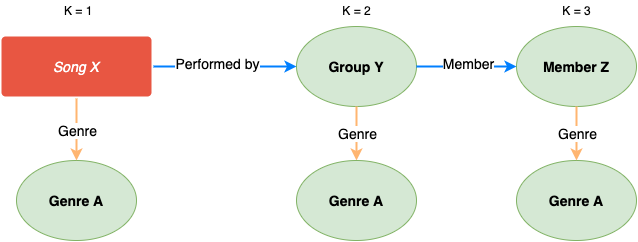
\includegraphics[width = 0.9\textwidth]{Imagenes/Bitmap/RelationLevels.png}
	\caption{Ejemplo de misma relación en distintos niveles}
	\label{fig:sampleImage}
\end{figure}

Para nuestro caso, en el cual tratamos con dos objetos iniciales que representan a dos canciones, hemos seleccionado una serie de propiedades a investigar para obtener los distintos niveles. El primer nivel es el más intuitivo: obtener relaciones directamente de ambas canciones. Entre esas relaciones se encontraría la relación ``Interpretado por'', la cual nos proporciona el artista o grupo que interpreta la canción. Este artista es el que vamos a usar como objeto de estudio del nivel k = 2, obteniendo así otro conjunto de relaciones del artista y sus respectivos valores. También obtendremos el género de la canción, que usaremos para generar el nivel k = 3 mediante las propiedades que obtengamos del género. Por último, como nivel final hemos seleccionado investigar las propiedades de los miembros que conforman la banda de música en caso de que el intérprete de la canción esté formado por varios artistas, y denominamos a este último nivel k= 4.\\

Queremos señalar que estos niveles podrían alargarse más a medida que seguimos investigando nuevas propiedades y generando un grafo más completo. Hemos decidido poner un límite en este punto debido a que, a medida que vamos avanzando en el estudio de los niveles de las propiedades, las explicaciones son menos significativas debido a que están más alejadas del primer nivel, que es el que está relacionado con la canción en sí.\\

En esta sección vamos a recopilar las principales propiedades de la lista total y cómo relacionarían dos canciones objeto iniciales. Algunas de ellas podrán aparecer en distintos niveles mientras que otras serán propias de un solo nivel:\\

\section{Explicaciones de la canción}

Aquí se encuentran las explicaciones basadas en propiedades del objeto canción que no pueden aparecer en el resto de niveles:

\subsection*{Artista}

El artista es una de las explicaciones más obvias pero también es una de las más importantes. Esta explicación hace referencia a cuando dos temas son interpretados por el mismo artista, por lo que tienen una clara relación directa ya que suele existir similitud entre las canciones de un artista. Además, a partir del artista podemos obtener otras relaciones más complejas en función de los datos de este mismo.\\

Como ejemplo podemos tomar los temas \textit{One More Time} y \textit{Something About Us}. Ambos son interpretados por el dúo musical \textbf{Daft Punk}, así que podemos explicar su relación gracias a este dato.\\

Para esta explicación utilizamos la propiedad ``performer''~(intérprete) de Wikidata. Siguiendo el modelo RDF, el sujeto es la canción (\textit{One More Time}, por ejemplo), el predicado es la propiedad intérprete y el objeto es el artista (\textbf{Daft Punk}).\\

\begin{figure}[h!]
	\centering
	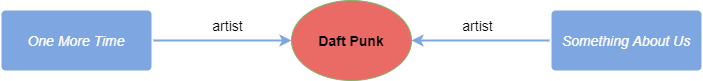
\includegraphics[width = 0.9\textwidth]{Imagenes/Bitmap/Artista ejemplo.png}
	\caption{Ejemplo de explicación por artista}
	\label{fig:sampleImage}
\end{figure}

\subsection*{Álbum}

Una explicación muy potente será que ambas canciones pertenezcan al mismo álbum. A menudo esta explicación aparecerá acompañada de la explicación del artista y, en cualquier caso, la relación que existe entre dos temas del mismo álbum suele ser más estrecha debido a que poseen más puntos en común, como puede ser el género, la fecha o la temática.\\

Tomemos como ejemplo \textit{Today} y \textit{Disarm}. Estas dos canciones son muy cercanas porque tienen varios puntos en común, pero una de las explicaciones que podemos ofrecer es que ambas pertenecen al álbum \textit{Siamese Dream}, de \textbf{The Smashing Pumpkins}. \textit{1979} es otro tema que se podría recomendar a raíz de \textit{Today}, pero es una peor elección que \textit{Disarm} porque pertenece a un álbum diferente.\\

Volvemos a utilizar Wikidata para obtener esta explicación, concretamente la propiedad ``part of''~(parte de). Esta propiedad se utiliza para varias cosas, entre ellas indicar los álbumes a los que pertenecen las canciones. Así obtenemos que \textit{Today} es ``parte de'' \textit{Siamese Dream}.\\

\begin{figure}[h!]
	\centering
	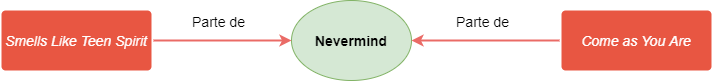
\includegraphics[width = 0.9\textwidth]{Imagenes/Bitmap/Álbum ejemplo.png}
	\caption{Ejemplo de explicación por álbum}
	\label{fig:sampleImage}
\end{figure}

\subsection*{Fecha de publicación (Década)}

Creemos que hay una mayor probabilidad de que exista una relación entre dos canciones que pertenezcan a la misma década. Esto se debe a que a lo largo del tiempo ha habido periodos marcados por uno o varios géneros musicales. Esto también ayuda a estudiar cómo estos distintos géneros están relacionados entre sí, lo cual es otro punto importante a tener en cuenta ya que hay géneros íntimamente relacionados entre sí: techno y house, heavy metal y thrash metal, etc.\\

Gracias a esta explicación, podemos relacionar dos canciones que a priori son muy distintas, como es el caso de \textit{Womanizer} de \textbf{Britney Spears} e \textit{Hysteria} de \textbf{Muse}. Estos temas no comparten algo tan básico como el artista o el género, pero ambos fueron publicados en los años 2000 y por ello pueden resultar interesantes para un usuario que busque escuchar los ritmos de esa época.\\

Para obtener esta explicación, emplearemos la propiedad ``publication date''~(fecha de publicación) de las canciones en Wikidata y comprobaremos si las dos fechas se sitúan dentro de la misma década.\\

\begin{figure}[h!]
	\centering
	\includegraphics[width = 0.9\textwidth]{Imagenes/Bitmap/Década ejemplo.png}
	\caption{Ejemplo de explicación por década}
	\label{fig:sampleImage}
\end{figure}

\subsection*{Singles}

Existe también una cierta relación entre aquellos temas que sean singles (o sencillos), así que consideramos esto como una explicación más. El razonamiento para esta decisión es que los singles son canciones que se publican de forma independiente por razones promocionales, por lo que suelen convertirse en los temas más populares y representativos del trabajo del artista. Por ello, pueden poseer más valor para el recomendador que otras canciones porque los singles tienen más probabilidades de coincidir con los gustos del usuario.\\

El tema \textit{Hung Up} de \textbf{Madonna} es un single, así que podemos establecer cierta relación con \textit{Feel Good Inc.} de \textbf{Gorillaz}, que también es un single.\\

Para esta explicación emplearemos la propiedad ``instance of''~(instancia de) en Wikidata y su valor ``single''. De esta forma comprobaremos que tanto \textit{Hung Up} como \textit{Feel Good Inc.} son ``instancia de'' ``single''.\\

\begin{figure}[h!]
	\centering
	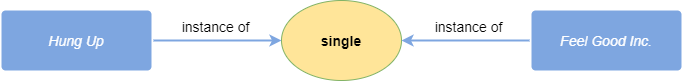
\includegraphics[width = 0.9\textwidth]{Imagenes/Bitmap/Single ejemplo.png}
	\caption{Ejemplo de explicación por single}
	\label{fig:sampleImage}
\end{figure}

\section{Explicaciones compartidas por Artista y Canción}

En esta sección exponemos propiedades que pueden ser establecidas tanto en el nivel de estudio de la canción como en el nivel de estudio del artista.

\subsection*{Premios}

La siguiente explicación son los premios recibidos. Existe una variedad de premios compartidos por diferentes canciones. Algunos de estos premios son más específicos que otros, pero en cualquier caso pueden resultar una relación útil para nuestras explicaciones ya que son un reflejo de la repercusión de las canciones. El mismo caso se da para los artistas, aquellos que suelen optar al mismo premio tienen más posibilidades de tener un estilo muy similar y por ende se puede establecer una relación de cercanía.\\

En esta sección hemos recogido dos propiedades: ``award received''~(premio recibido) y ``nominated for''~(nominado a). Estas categorías hacen referencia a los premios que han recibido los artistas o canciones y a los premios a los que han sido nominados respectivamente. Normalmente los premios se reparten según distintas categorías en función al estilo de música, pero también hay otros que nos aportan otro tipo de información al estudio como Grammy al Mejor Videoclip, Grammy Award a la Mejor Canción Escrita, Grammy Award a la Mejor Interpretación Rap/Sung etc...\\

Basándonos en el nivel de canción tenemos como ejemplo \textit{Single Ladies (Put a Ring on It)} de \textbf{Beyoncé} y \textit{Rolling in the Deep} de \textbf{Adele}, ya que ambos temas han recibido el Premio Grammy a la canción del año. Además, como es lógico, ambas canciones fueron nominadas a ese mismo premio, así que podemos mostrar ambas propiedades en este ejemplo.\\

Usaremos la propiedad ``award received''~(premio recibido) y ``nominated for''~(nominado a) encontradas en Wikidata. De esta forma, \textit{Rolling in the Deep} sería el sujeto, ``award received'' y ``nominated for'' serían los predicados y \textit{Grammy Award for Song of the Year} sería el objeto.\\

\begin{figure}[h!]
	\centering
	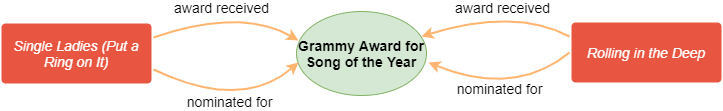
\includegraphics[width = 0.9\textwidth]{Imagenes/Bitmap/Premio ejemplo.png}
	\caption{Ejemplo de explicación por premio}
	\label{fig:sampleImage}
\end{figure}

\subsection*{Género}

La explicación Género es una de las más representativas ya que las personas se guían por el género que prefieren para escuchar canciones similares, aunque en ocasiones no deba ser así. Un usuario que sea fan del jazz querrá escuchar canciones de ese mismo género o géneros similares porque todas los temas de un mismo género comparten una serie de puntos en común como la elección de los instrumentos, temáticas similares en sus letras o patrones de composición.\\

Gracias al género, podemos explicar la relación entre canciones como \textit{A-Punk} de \textbf{Vampire Weekend} e \textit{Brianstorm} de \textbf{Arctic Monkeys}, que pertenecen a un subgénero muy concreto del rock conocido como \textbf{surf music}.\\

Para esta relación utilizamos la propiedad ``genre''~(género) de Wikidata. Así tenemos que la canción \textit{A-Punk} pertenece al género \textbf{surf music}.\\

\begin{figure}[h!]
	\centering
	\includegraphics[width = 0.9\textwidth]{Imagenes/Bitmap/Género ejemplo.png}
	\caption{Ejemplo de explicación por género entre canciones}
	\label{fig:sampleImage}
\end{figure}

En este caso podríamos crear una relación del mismo tipo con los artistas, debido a que ambos artistas de las dos canciones previas también cuentan con un registro de \textbf{alternative rock} (entre otros géneros) en su propiedad de género.\\

\begin{figure}[h!]
	\centering
	\includegraphics[width = 0.9\textwidth]{Imagenes/Bitmap/Género ejemplo artistas.png}
	\caption{Ejemplo de explicación por género entre artistas}
	\label{fig:sampleImage}
\end{figure}

\subsection*{Idioma}

La explicación Idioma denota, como su nombre sugiere, que ambas canciones están en el mismo idioma o lenguaje. Existen numerosos ejemplos de temas musicales que están escritos en un idioma que no se corresponde con la lengua materna del artista que los publican, o sencillamente están escritas en un idioma que se habla en varias partes del mundo distintas, como el inglés o el español. En ciertos casos el compartir idioma es un indicativo de otras relaciones adicionales, como puede ser el caso de canciones que pertenecen a un folclore regional determinado. En cualquier caso el compartir lenguaje ya es una relación directa en sí misma.\\

Como ejemplo podemos tomar el tema \textit{Talk} de \textbf{Coldplay} y \textit{Light My Fire} de \textbf{The Doors}, los cuales están escritos en inglés.\\

Para esta explicación emplearemos la propiedad ``language of work or name''~(idioma de la obra o del nombre) de Wikidata. Así tenemos que la canción \textit{Talk} tiene idioma ``inglés''.\\

\begin{figure}[h!]
	\centering
	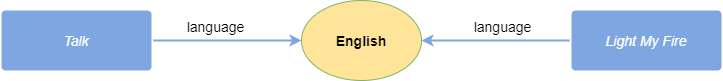
\includegraphics[width = 0.9\textwidth]{Imagenes/Bitmap/Idioma ejemplo.png}
	\caption{Ejemplo de explicación por idioma}
	\label{fig:sampleImage}
\end{figure}

La misma explicación podría para relacionar dos artistas con una misma propiedad de idioma, lo que significa que ambos artistas han trabajado interpretando canciones en ese idioma.\\

\section{Explicaciones compartidas por Canción, Artista y Miembro}

En esta sección solo aparecen las principales propiedades que por naturaleza son exclusivas de la canción, el artista o un miembro del grupo (en caso de que el artista sea una banda compuesta por varias personas).\\

\subsection*{Compañía discográfica}

Record Label~(compañía discográfica) hace referencia a la compañía por la que ha firmado el artista para publicar un tema concreto. Hemos podido observar que una misma compañía puede firmar a artistas que a veces no tienen relación ninguna en cuanto al estilo musical, pero hay otras causas que sí los pueden relacionar indirectamente como la tendencia del momento, el target del público que generan, etc. También se puede dar el caso en el que un miembro del grupo firme o haya firmado con una compañía individual, ya sea por conceptos relacionados con marcas, representantes o contratos. Además también tenemos en cuenta la compañía discográfica bajo la que se ha publicado cada canción, lo cual nos puede aportar relaciones adicionales.\\

Para ilustrarlo con un ejemplo, las canciones \textit{Personal Jesus} de \textbf{Depeche Mode} y \textit{Australia} de \textbf{The Shins} pertenecen a bandas que han trabajado con el sello discográfico \textbf{Columbia Records}.\\

Podemos alcanzar esta explicación gracias a la propiedad ``record label''~(sello discográfico) de Wikidata. \textit{Personal Jesus} tiene un ``record label'' cuyo nombre (o valor) es \textbf{Columbia Records}.\\\\\

\begin{figure}[h!]
	\centering
	\includegraphics[width = 0.9\textwidth]{Imagenes/Bitmap/Discográfica ejemplo.png}
	\caption{Ejemplo de explicación por compañía discográfica}
	\label{fig:sampleImage}
\end{figure}

\section{Explicaciones compartidas por Género, Artista y Miembro}

Estas explicaciones son compartidas por géneros, artistas y miembros, excluyendo solamente el nivel de canción.\\

\subsection*{Lugar de formación}

La propiedad ``location of formation''~(lugar de formación) que hace referencia a la localidad de formación del grupo o artista, puede parecer muy similar a la explicación ``country of origin'', pero esta ejerce una selección más precisa porque nos da un núcleo de población más pequeño. Un ejemplo de ello podrían ser dos míticas bandas de la ciudad de Seattle: \textbf{Pearl Jam} y \textbf{Foo Fighters}. Creemos que la unión de la ciudad natal con la música puede hacer a un usuario el escuchar grupos de su misma ciudad o estado. En cuanto a la relación referente a un miembro del grupo, se trataría del lugar donde ese miembro se inició como músico ya sea como artista en solitario o en su grupo original.\\

De esta forma podemos explicar la relación existente entre sus temas \textit{Black} y \textit{Everlong}, respectivamente.\\

\begin{figure}[h!]
	\centering
	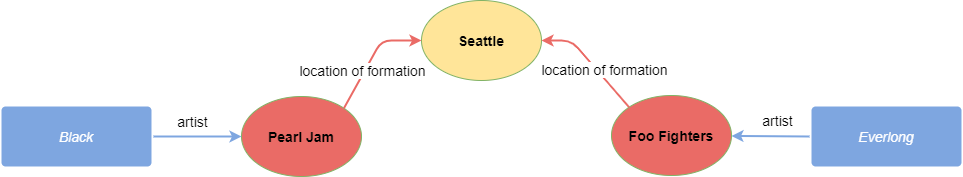
\includegraphics[width = 0.9\textwidth]{Imagenes/Bitmap/LocationOfFormation.png}
	\caption{Ejemplo de explicación por lugar de formación}
	\label{fig:sampleImage}
\end{figure}

\section{Explicaciones compartidas por Artista, Miembro, Género y Canción}

Estas explicaciones son compartidas en los cuatro niveles y resultan de gran interés porque nos permitirán enlazar los cuatro mismos en el caso en el que coincidan en el objeto con las relaciones de la canción opuesta.\\

\subsubsection*{País de origen}

Esta explicación puede ser especialmente útil para países relativamente pequeños donde la música nacional presenta unos patrones claros. Además, a lo largo de la historia en un país se genera una tendencia o nuevo género musical el cual es propio de ese país en el que se forma un artista y esto nos daría una relación muy específica que definitivamente acertaría por completo en la relación 1 a 1 de dos canciones.\\

En países que son significativamente grandes o con una población muy alta perdería algo de especificidad, pero aún así hay más posibilidades de que dos un artistas del mismo país sean escuchados por un mismo usuario.\\

La canción \textit{Black Hole Sun} de la banda \textbf{Soundgarden} y \textit{Closer} de \textbf{Nine Inch Nails} guardan cierta similitud porque ambos grupos son originarios de \textbf{Estados Unidos}.\\

Para comprobarlo, obtendremos la propiedad ``country of origin''~(país de origen) del artista que previamente ya hemos almacenado al estudiar las relaciones directas en el caso de las bandas o la propiedad ``country of citizenship''~(país de nacionalidad) en el caso de los artistas en solitario. \textit{Black Hole Sun} tiene el ``performer'' \textbf{Soundgarden}, cuyo ``country of origin'' es \textbf{United States of America}.\\

\begin{figure}[h!]
	\centering
	\includegraphics[width = 1\textwidth]{Imagenes/Bitmap/País ejemplo.png}
	\caption{Ejemplo de explicación por país de origen}
	\label{fig:sampleImage}
\end{figure}

También podemos recoger la información del país donde se formó ese género. Con esta propiedad queremos recoger movimientos artísticos que surgieron en el mismo país. Los géneros que fueron formados en un determinado país están mucho más arraigados a este a pesar de que se hayan extendido por todo el mundo. Es por esto que si queremos relacionar una artista que cualquier parte del mundo, que tiene un estilo techno, será más propenso a estar relacionado con artistas o canciones holandesas, cuna de este estilo musical.\\

En el caso de que la propiedad se estableciese en la canción, significaría que ambas canciones han sido lanzadas originariamente en el mismo país.\\

\subsubsection*{Influenciado por}

La \textbf{influencia de los artistas} es otra explicación importante. A menudo el trabajo de un artista se ve influenciado por otros artistas de formas que no siempre están ligadas a un género musical concreto, así que podemos encontrar una relación entre dos canciones examinando estas influencias.\\

Tomando como ejemplo las canciones \textit{Billie Jean} de \textbf{Michael Jackson} y \textit{Paint It Black} de \textbf{The Rolling Stones}, podemos establecer una relación entre ellas al ver que ambos artistas fueron influenciados por la banda \textbf{The Beatles}.\\

Obtenemos esta explicación gracias a la propiedad ``influenced by''~(influenciado por) de Wikidata, además de la propiedad ``performer'' para relacionar el tema con su artista. Así averiguamos que \textit{Billie Jean} tiene de ``intérprete'' a \textbf{Michael Jackson}, quien fue ``influenciado por'' \textbf{The Beatles}.\\

\begin{figure}[h!]
	\centering
	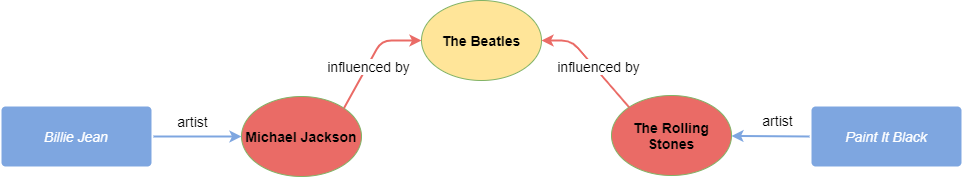
\includegraphics[width = 1\textwidth]{Imagenes/Bitmap/Influencia ejemplo.png}
	\caption{Ejemplo de explicación por influencia}
	\label{fig:sampleImage}
\end{figure}

Al igual que con el artista, los géneros también son influenciados por otros los cuales ha servido para el desarrollo de nuevos estilos a lo largo de la historia. Gracias a la evolución del Rock hay otros géneros que han marcado tendencia como el Rock and Roll, el Heavy Metal,Hard Rock, Garage Rock etc...\\

\section{Propiedades propias del artista o grupo}

Aquí se expones las principales relaciones que solo pueden ser propias del artista o grupo.\\

\subsubsection*{Integrantes}

Los \textbf{integrantes} son cada uno de los miembros que conforman un grupo. En caso de ser un único artista, esta propiedad es irrelevante ya que haríamos referencia a la propiedad directa de artista. Esta propiedad resulta útil en casos en los que miembros de la banda han cambiado de grupo a lo largo de su carrera musical. Esto nos da acceso a otros grupos que por valores o gustos musicales del artista nos hacen pensar que pueden ser muy parecidos.\\

Si tomamos los temas \textit{Lithium} de \textbf{Nirvana} y \textit{Everlong} de \textbf{Foo Fighters} podemos observar que existe una relación entre ellos porque el músico \textbf{Dave Grohl} ha formado parte de ambas bandas.\\

Para comprobarlo usaremos la propiedad de Wikidata ``performer'' y después comprobaremos la propiedad ``has part''~(compuesto de) para ver todos los miembros de la banda y buscar coincidencias. De este modo, podemos ver que \textit{Everlong} tiene un ``performer'' que es \textbf{Foo Fighters}, y a su vez \textbf{Foo Fighters} ``has part'' \textbf{Dave Grohl}.\\\\\\

\begin{figure}[h!]
	\centering
	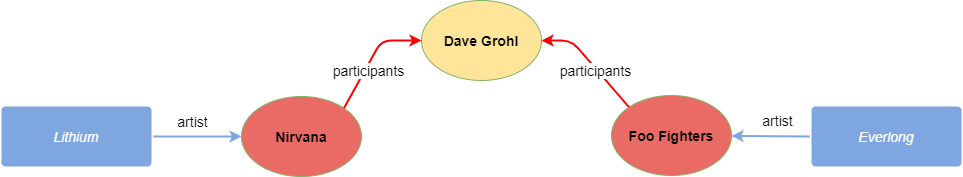
\includegraphics[width = 0.8\textwidth]{Imagenes/Bitmap/Integrante ejemplo.png}
	\caption{Ejemplo de explicación por integrantes}
	\label{fig:sampleImage}
\end{figure}

\subsubsection*{Tipo de voz}

Siguiendo con el estudio de los artistas, el \textbf{tipo de voz} de los vocalistas es una buena explicación para relacionar dos canciones. El tipo de voz influye en el sonido general del tema y puede ser especialmente determinante en ciertos géneros musicales. Por limitaciones técnicas, solo aplicaremos esta explicación con artistas en solitario.\\

La voz de un artista puede encajar en más de un tipo, aunque en esta explicación buscamos que coincidan en al menos un tipo. La cantante \textbf{Lady Gaga} se asemeja a \textbf{Amy Winehouse} por su tipo de voz, ya que ambas son \textit{mezzo-soprano}. Así podemos explicar la relación entre dos canciones de estas artistas como \textit{Poker Face} y \textit{Rehab}.\\

Para esta explicación resulta útil la propiedad ``voice type''~(tipo de voz) en Wikidata. Partiendo de \textit{Poker Face}, utilizamos la propiedad ``performer'' para llegar a \textbf{Lady Gaga} y finalmente usamos su ``voice type'' para obtener \textit{mezzo-soprano}.\\

\begin{figure}[h!]
	\centering
	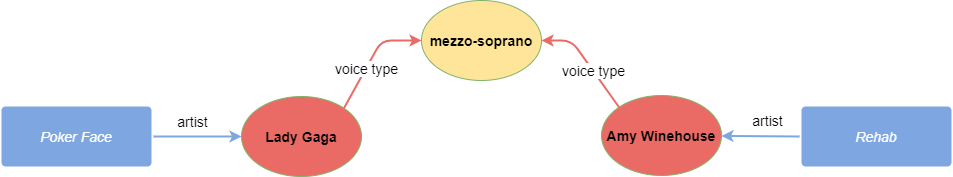
\includegraphics[width = 1\textwidth]{Imagenes/Bitmap/Voz ejemplo.png}
	\caption{Ejemplo de explicación por tipo de voz}
	\label{fig:sampleImage}
\end{figure}

\subsubsection*{Fecha de fundación}

Con esta propiedad intentamos tener en cuenta la historia de los o su cronograma. Hay grupos que comenzaron su etapa musical  conjuntamente a lo largo del tiempo. Un ejemplo de este caso se en curiosamente en el technopop que tanto caracterizó a los años 80, pues convivió a veces con el soul y con el estilo afroamericano doo-wop.\\

Gracias a esta explicación podemos relacionar canciones como \textit{Clint Eastwood} de \textbf{Gorillaz} y \textit{Parabola} de \textbf{Tool}. Son canciones muy diferentes, pero ambos artistas comenzaron su carrera en la década de los 90, por lo que comparten un marco temporal.\\

Utilizaremos la propiedad ``work period (start)''~(inicio del periodo de actividad) de Wikidata para obtener esta explicación. \textit{Clint Eastwood} tiene de intérprete a \textbf{Gorillaz}, que a su vez inició su periodo de actividad en la década de los 90.\\

\begin{figure}[h!]
	\centering
	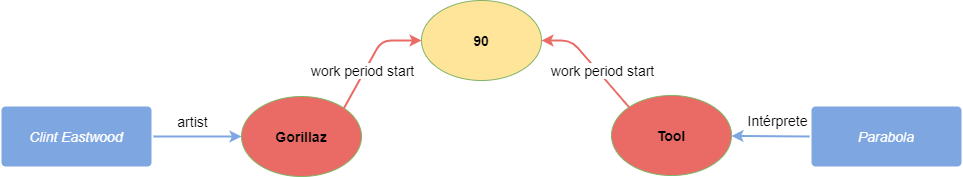
\includegraphics[width = 1\textwidth]{Imagenes/Bitmap/Fundacion ejemplo.png}
	\caption{Ejemplo de explicación por fecha de fundación}
	\label{fig:sampleImage}
\end{figure}

\section{Explicaciones basadas en el género}

Estas propiedades vienen ligadas directamente al género de la canción. Es una de las propiedades más detalladas en Wikidata y por lo tanto una de de las que más información nos pueden proporcionar. Hay muchos géneros y subgéneros documentados, lo que nos facilita la obtención y clasificación de estos.\\

\subsection{Subgénero}

Cabe destacar la diferencia entre las propiedades ``Influenciado por'' y ``Subgénero''; mientras que la primera solo indica que ese estilo musical ha marcado una cierta influencia tomando algunos aspectos, la segunda señala que es un Subgénero, una tendencia muy parecida y que toma como base ese estilo musical.\\

De esta forma podemos explicar la cercanía existente entre dos canciones como \textit{One} de \textbf{Metallica} y \textit{Schism} de \textbf{Tool}. La primera canción pertenece al género \textbf{thrash metal} mientras que la segunda es un ejemplo de \textbf{progressive metal} y, a su vez, ambos géneros son subgéneros del \textbf{heavy metal}.\\

Para esta explicación usamos la propiedad ``subclass of''~(subclase de) encontrada en Wikidata. Así tenemos que \textit{One} pertenece al género \textbf{thrash metal}, el cual es ``subclass of'' \textbf{heavy metal}.\\

\begin{figure}[h!]
	\centering
	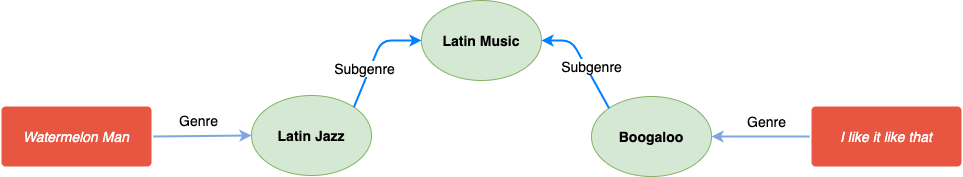
\includegraphics[width = 1\textwidth]{Imagenes/Bitmap/Subgenre.png}
	\caption{Ejemplo de explicación por Subgénero}
	\label{fig:sampleImage}
\end{figure}


